\documentclass{beamer}
\setbeamertemplate{navigation symbols}{}

\usepackage{hyperref}
\usepackage{dirtytalk}
\usepackage{emoji}
\usepackage[utf8]{inputenc}
\usepackage[
  english,
  spanish,
  es-tabla,
  es-nodecimaldot
]{babel}
\selectlanguage{spanish}
\usepackage{minted}
\setminted[python]{frame=single,autogobble,linenos,numbersep=4pt,fontsize=\footnotesize}

\usetheme{Rochester}
\definecolor{pinky}{rgb}{0.9098, 0.2627, 0.4431}
\usecolortheme[named=pinky]{structure}

\title{{\Huge\emoji{technologist-light-skin-tone}}\\¡Comenzando con Python!}
\author{Sergio García Prado}
\date{\today}

\begin{document}

    \begin{frame}
        \titlepage
    \end{frame}

    \begin{frame}{Sobre mi}
      \noindent
      \begin{minipage}{.24\textwidth}
          \begin{figure}
            \centering
            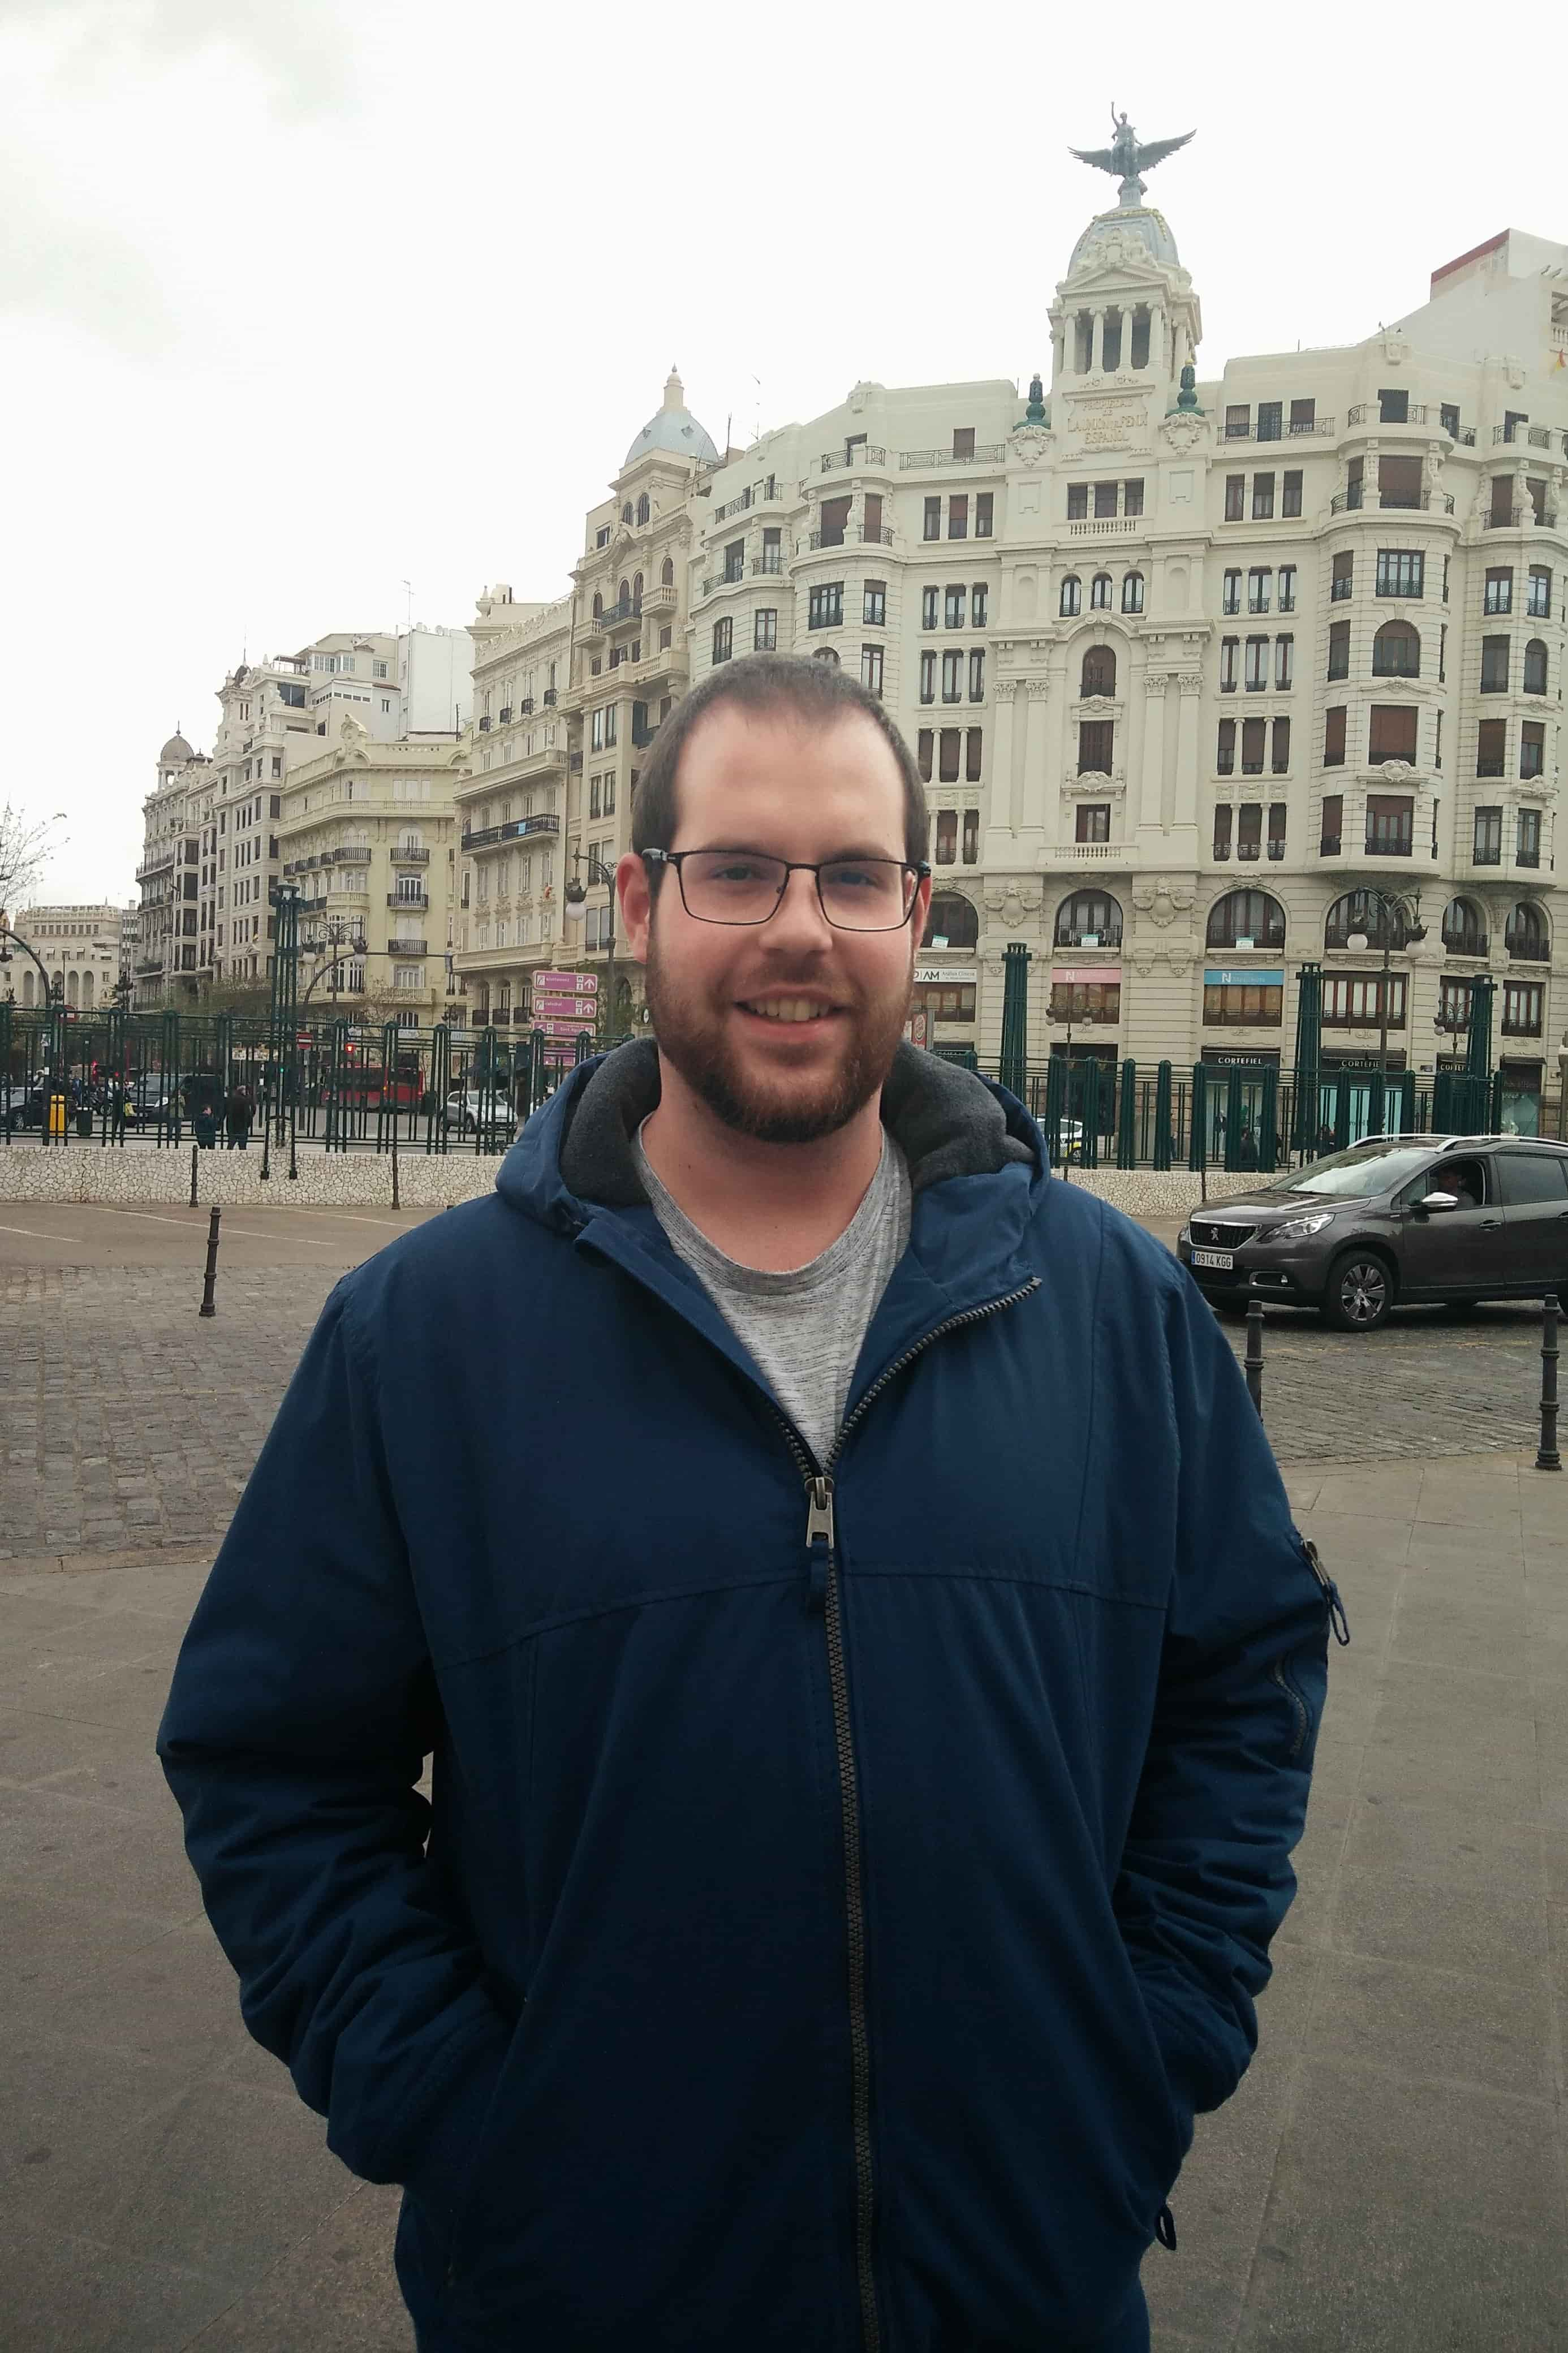
\includegraphics[width=\textwidth]{images/photo}
          \end{figure}
      \end{minipage}
      \begin{minipage}{.74\textwidth}
          \begin{itemize}
            \item ¡Hola! Soy Sergio García Prado
            \item Estudios:
            \begin{itemize}
              \item \emoji{desktop-computer} Graduado en Ingeniería Informática
              \item \emoji{chart-increasing} Graduado en Estadística
            \end{itemize}
            \item Experiencia Laboral:
            \begin{itemize}
              \item \emoji{rocket} Trabajando en Unlimiteck
            \end{itemize}
            \item Sígueme:
                \begin{itemize}
                    \item Website: \href{http://garciparedes.me}{garciparedes.me}
                    \item GitHub: \href{http://github.com/garciparedes}{@garciparedes}
                    \item Email: \href{mailto:sergio@garcipardes.me}{sergio@garcipardes.me}
                \end{itemize}
          \end{itemize}
      \end{minipage}
    \end{frame}

    \begin{frame}{¿Qué es programar?}
      \noindent
      \begin{minipage}{.69\textwidth}
          \say{La programación es el proceso utilizado para idear y ordenar las acciones necesarias para realizar un proyecto, preparar ciertas máquinas o aparatos para que empiecen a funcionar en el momento y en la forma deseados o elaborar programas para su empleo en computadoras}
          \rightline{{\rm ---  R.A.E. (2014)}}
      \end{minipage}
      \begin{minipage}{.29\textwidth}
          \begin{center}
            \fontsize{40}{50}
              \emoji{computer}
          \end{center}
      \end{minipage}
    \end{frame}

    \begin{frame}{Similitud con recetas de cocina}
        \noindent
        \begin{minipage}{.29\textwidth}
          \begin{center}
            \fontsize{40}{50}
              \emoji{cake}
          \end{center}
        \end{minipage}
        \begin{minipage}{.69\textwidth}
            \begin{itemize}
                \item La idea de programar sobre un ordenador no es muy diferente de la tareas como la de seguir una receta.
                \item Receta de Bizcocho:
                \begin{enumerate}
                    \item Mezclar ingredientes secos.
                    \item Mezclar ingredientes húmedos.
                    \item Combinar todos los ingredientes.
                    \item Encender el horno.
                    \item Amasar hasta conseguir una masa homogénea.
                    \item Hornear durante 30 minutos.
                    \item Dejar reposar.
                \end{enumerate}
            \end{itemize}
        \end{minipage}
    \end{frame}

    \begin{frame}{Pensamiento jerárquico: desde arriba hasta abajo}
        \begin{itemize}
          \item La idea de la programación se basa en la construcción de abstracciones sobre conceptos básicos, que de manera conjunta forman una base de conocimiento más rica.
          \item Ejemplo:
          \begin{itemize}
            \item Hacer bizcocho
            \item Mezclar ingredientes secos, ...
            \item Mezclar harina, azúcar, levadura, ...
            \item Introducir harina en el recipiente, introducir azúcar en el recipiente, ...
            \item Abrir paquete de harina, calcular cantidad de harina, ...
            \item ...
          \end{itemize}
        \end{itemize}
    \end{frame}

    \begin{frame}{¡Hola, Mundo!}
      \noindent
      \begin{minipage}{.69\textwidth}
        \begin{itemize}
          \item El término \emph{Hello, World} consiste en la ejemplificación sobre las sentencias necesarias para un lenguaje de programación determinado, de tal manera que este imprima por consola el texto \texttt{Hello, World!}.
          \item Hola mundo en \emph{Python}: \mintinline{python}{print("Hello, World!")}
        \end{itemize}
      \end{minipage}
      \begin{minipage}{.29\textwidth}
          \begin{center}
            \fontsize{40}{50}
              \emoji{man-raising-hand-light-skin-tone}\emoji{earth-africa}
          \end{center}
      \end{minipage}
    \end{frame}

    \begin{frame}{¿Por qué Python es popular?}
        \noindent
        \begin{minipage}{.29\textwidth}
            \begin{center}
              \fontsize{40}{50}
                \emoji{snake}
            \end{center}
        \end{minipage}
        \begin{minipage}{.69\textwidth}
          \begin{itemize}
            \item \emph{Python} es un lenguaje de programación interpretado cuya filosofía hace hincapié en la \emph{legibilidad de su código}.​ bu
            \item En los últimos años ha sufrido un crecimiento exponencial, entre otros, por el ecosistema de tan heterogéneo que se ha ido construyendo a su alrededor: \emph{Data Science}, \emph{Web Development}, \emph{Embedded Systems}, etc.
          \end{itemize}
        \end{minipage}
    \end{frame}

    \begin{frame}{Caso Práctico: Recordatorios}
        \noindent
        \begin{minipage}{.69\textwidth}
          \begin{itemize}
            \item [TODO]
          \end{itemize}
        \end{minipage}
        \begin{minipage}{.29\textwidth}
            \begin{center}
              \fontsize{40}{50}
                \emoji{memo}
            \end{center}
        \end{minipage}
    \end{frame}

    \begin{frame}[fragile]{Python Sample}
        This is a text in the first frame.
        \begin{figure}
            \begin{minipage}[c]{0.7\textwidth}
                \begin{minted}{python}
                    def main():
                      print("hello")

                    if __name__ == '__main__':
                      main()
                \end{minted}
            \end{minipage}
        \end{figure}
    \end{frame}


    \begin{frame}
        \begin{center}
            \Huge
            ¿Preguntas?
        \end{center}
    \end{frame}
\end{document}
